\documentclass[dvipdfmx]{jsarticle}
\usepackage{tikz,ascmac,amsmath,amssymb,amsthm,bm,physics,arydshln,mathcomp,wrapfig,pgfplots,multicol}
\usetikzlibrary{calc}
\usetikzlibrary{intersections}
\DeclareMathOperator{\id}{id} %\idは定義されていない
\newtheorem*{answer*}{解答}

\begin{document}
\textbf{問1} \ $U, V$ をそれぞれ$\mathbb{R}^m$, $\mathbb{R}^n$ の開集合とする. 
写像$f: U \to V$ の座標表示を$f = (f_1, ......, f_n)$ とする.

\ \ \ \ \ このとき, 次の(i), (ii) が同値であることを示せ.

\ \ \ \ \ (i) $f: U \to V$ は連続写像である.

\ \ \ \ \ (ii) 各$i=1, ......, n$ に対して $f_i: U \to \mathbb{R}$ が連続関数.

\bigskip

\textbf{問2} \ 位相多様体$M$は局所弧状連結空間であることを示せ.

\bigskip

\textbf{問3} \ 位相多様体$M$ は局所コンパクトであることを示せ.

\bigskip

\textbf{問4} \ 

(1) \ $GL(n,\mathbb{R})$ が$n^2$次元可微分多様体となることを示せ.

(2) \ $C^{\infty}$ 級多様体 $GL(n, \mathbb{R})$ の各元 $A$ を逆行列$A^{-1}$ に対応させる写像 $g : GL(n, \mathbb{R}) \to GL(n, \mathbb{R})$, \ $g(A) = A^{-1}$ が $C^{\infty}$ 級写像であることを示せ.

\bigskip

\textbf{問5} \ $\mathbb{R}^n$ の開集合$U$ と$C^{\infty}$級関数$f: U \to \mathbb{R}^m$ に対して, 

$f$ のグラフ $\Gamma(f) = \{(\bm{x}, f(\bm{x})) | \ \bm{x} \in U\}$ が$n$次元$C^{\infty}$級多様体となることを示せ.

\bigskip

\textbf{問6} \ 次の位相空間は位相多様体となるか.

(1) $M = \{(x,y) \in \mathbb{R}^2 | \ y = |x| \}$

(2) $M = \{(x,y) \in \mathbb{R}^2 | \ y = |x| \} \cup
         \{(x,y) \in \mathbb{R}^2 | \ y = -|x| \}$

(3) $M = \{(x,y) \in \mathbb{R}^2 | \ xy = 0\}$

\bigskip

\textbf{問7} \ $1$次元Euclid空間$\mathbb{R}$の開集合$U, V$ を$U:= (-\infty, 1), V:= (1, \infty)$ で定め, $2$つの写像

 \ \ \ \ $\id_U : U \to U$ \ 恒等写像

 \ \ \ \ \ \ \ $f : V \to V \ x \mapsto x^3$ \ \ と定義する.

このとき, 集合族$\{(U, \id_U), \ (V, f) \}$ は$\mathbb{R}$ の座標近傍系であるが, 

$C^{\infty}$級座標近傍系にはならないことを示せ.

\bigskip

\textbf{問8} \ 
同値でない$C^{\infty}$ 級座標近傍系の例を挙げよ.

\bigskip

\textbf{問9} \ 
$C^r$ 級多様体 $M$ の$2$ つの $C^r$ 級座標近傍系$\mathcal{S}$ と $\mathcal{T}$ に対して次のような関係を定める.

$$
\mathcal{S} \sim \mathcal{T} \Longleftrightarrow
\mathcal{S} と \mathcal{T} が同値
$$

このとき, この関係$\mathcal{S} \sim \mathcal{T}$ は同値関係であることを示せ.


\bigskip
\bigskip

[\textbf{解答}]

\textbf{問1}

(i) $\Longrightarrow$ (ii)

任意の$a \in U, \ \varepsilon > 0$ を取る. $f$ は連続写像なので, $\exists \delta > 0$ s.t. $d(x,a) < \delta \Longrightarrow d^n(f(x),f(a) < \varepsilon$ なので 

$d(x,a) < \delta$ のとき
$d(f_i (x), f_i (a)) = \sqrt{(f_i (x) - f_i (a))^2} \leqq \sqrt{\displaystyle\sum_{i=1}^n (f_i (x) - f_i (a))^2} = d^n (f(x), f(a)) < \varepsilon$ となり$f_i$ は連続.

(ii) $\Longrightarrow$ (i)

任意の$a \in U, \ \varepsilon > 0$ をとる. 仮定より$f_i$ は連続関数なので 

$\exists \delta_i > 0$ s.t. $d(x,a) < \delta_i \Longrightarrow d(f_i (x), f_i (a)) < \displaystyle\frac{\varepsilon}{n}$. 

よって$\delta:= \min\{\delta_1, ......, \delta_n\}$ とすると, $d(x,a) < \delta$ のとき, 

$d^n (f(x), f(a)) = \sqrt{\displaystyle\sum_{i=1}^n (f_i (x)-f_i(a))^2} \leqq \displaystyle\sum_{i=1}^n d(f_i (x), f_i (a)) < n \cdot \frac{\varepsilon}{n} = \varepsilon$

\bigskip

\textbf{問2}

$M$ の任意の点$x$の任意の開近傍$U_x$ を考える. そして$M$ を$n$次元位相多様体とすると$\mathbb{R}^n$ のある開集合$V$と同相な$x$ のある開近傍$V_x$ が存在する. このとき$U_x \cap V_x$ を考えるとこれも$x$ の開近傍であるから, 同相写像$\varphi: V_x \to V$ を定めると開写像の定義より$\varphi(U_x \cap V_x)$ は$V$ の開集合であり, 
$B^n (\varphi(x) ; \varepsilon) \subset \varphi(U_x \cap V_x) \subset V$ となるようなある正の実数$\varepsilon$が存在する.

このとき, $x \in \varphi^{-1} (B^n(\varphi(x) ; \varepsilon)) \subset U_x \cap V_x \subset U_x$ であり, $\mathbb{R}^n$ の開球$B^n (\varphi(x) ; \varepsilon)$ は弧状連結. よってその連続像$\varphi^{-1} (B^n(\varphi(x) ; \varepsilon)) $ も弧状連結.
したがって, $M$ は局所弧状連結空間である.

\bigskip

\textbf{問3}

$M$ をn次元位相多様体とすると, 任意の$x \in M$ に対して写像$\varphi: U_x \to V$ が同相写像となるような$x$ の開近傍$U_x$, $\mathbb{R}^n$ の開集合$V$ が存在する. $\mathbb{R}^n$ は局所コンパクト空間なので, $\varphi(x)$ のコンパクトな近傍$V_{\varphi(x)}$ が存在する. このとき, $V_{\varphi(x)}^i \cap V$ は$V$ の開集合なので, $\varphi(x) \in \overline{B^n}(\varphi(x) ; \varepsilon) \subset V_{\varphi(x)}^i \cap V$ となるような正の実数$\varepsilon$ が存在する. $\overline{B^n}(\varphi(x) ; \varepsilon)$ は$\varphi(x)$ の近傍であり, 当然$\varphi(x) \in B^n(\varphi(x) ; \varepsilon)$ となるので, 
$x \in \varphi^{-1} (B^n(\varphi(x) ; \varepsilon)) \subset \varphi^{-1} (\overline{B^n}(\varphi(x) ; \varepsilon))$
となる. $\varphi$ は連続写像なので $\varphi^{-1} (B^n(\varphi(x) ; \varepsilon))$ は$U_x$ の開集合であり,
$x \in \varphi^{-1} (B^n(\varphi(x) ; \varepsilon)) 
= (\varphi^{-1} (B^n(\varphi(x) ; \varepsilon)))^i
\subset (\varphi^{-1} (\overline{B^n}(\varphi(x) ; \varepsilon)))^i$ が得られる.
よって$\varphi^{-1} (\overline{B^n}(\varphi(x) ; \varepsilon))$ は$x$ の近傍であり, コンパクト空間の連続像はコンパクト空間となるので $\varphi^{-1} (\overline{B^n}(\varphi(x) ; \varepsilon))$ は $x$ のコンパクトな近傍となる.

したがって, $M$ は局所コンパクト空間である.

\bigskip

\textbf{問4}

＜方針＞

$M(n, \mathbb{R})$ と$\mathbb{R}^{n^2}$ の間の同相写像を構成することにより$M(n, \mathbb{R})$ が$C^{\infty}$級多様体であることを示し,

$GL(n, \mathbb{R})$ が$M(n, \mathbb{R})$ の開部分多様体となることを言う.

\bigskip

$A = (a_{ij})_{1\leqq i, j \leqq n} \in M(n, \mathbb{R})$ とし, 
写像
\[\begin{array}{rccc}
\varphi \colon & M(n, \mathbb{R}) & \longrightarrow & \mathbb{R}^{n^2} \\
        & \rotatebox{90}{$\in$} & & \rotatebox{90}{$\in$} \\
        & A & \longmapsto & \bm{a}
\end{array}\]

\begin{flushright}
($\bm{a} := (a_{11}, a_{12}, ......, a_{1n}, a_{21}, ......, a_{2n}, ......., a_{n1}, ......, a_{nn})$)  
\end{flushright}

を定めると, 
任意の$\bm{a} \in \mathbb{R}^{n^2}$ に対して $\bm{a}$ の各成分を行列の各成分に対応させることにより行列$A$ がただ一つに定まるので$\varphi$ は全単射.
($\varphi$ との合成が$\id_{M(n, \mathbb{R})}, \ \id_{\mathbb{R}^{n^2}}$ になるような逆写像の存在を示しても良い)

次に, 集合系$\mathcal{O}_{M(n, \mathbb{R})} := \{\varphi^{-1}(O) | \ O \in \mathcal{O}_{\mathbb{R}^{n^2}}\}
= \{O' \subset M(n, \mathbb{R}) | \ \varphi(O') \in \mathcal{O}_{\mathbb{R}^{n^2}} \}$ を定めると, これは$M(n, \mathbb{R})$ の位相であり$\varphi$ は連続かつ開写像となる.

よって$\varphi$ は同相写像.

$M(n, \mathbb{R})$ が$n^2$次元$C^{\infty}$級多様体になることを示していく.

(i)

$\mathbb{R}^{n^2}$ はハウスドルフ空間なので, $\mathbb{R}^{n^2}$ と同相な$M(n, \mathbb{R})$ もハウスドルフ空間.

\bigskip

(ii)

$M(n,\mathbb{R})$ は$1$つの$n^2$次元チャートからなるアトラス$\{(M(n, \mathbb{R}), \varphi)\}$ を持つ.

\bigskip

(iii)

$1$つのチャート$(M(n, \mathbb{R}), \varphi)$ に対して, 座標変換$\varphi \circ \varphi^{-1} = \id_{\mathbb{R}^{n^2}}$ は明らかに$C^{\infty}$級写像.

\bigskip

(i)～(iii)より, $M(n, \mathbb{R})$ は$n^2$次元$C^{\infty}$級多様体.

次に, $GL(n, \mathbb{R}) \subset M(n, \mathbb{R})$ が$M(n, \mathbb{R})$ の開集合になっていることを示す.

まず, 行列式関数
\[\begin{array}{rccc}
f \colon & M(n, \mathbb{R}) & \longrightarrow & \mathbb{R} \\
        & \rotatebox{90}{$\in$} & & \rotatebox{90}{$\in$} \\
        & A & \longmapsto & \det(A)
\end{array}\]
を定めると, $f$ は連続写像である.

$\left(  \begin{tabular}{l}
$\because f = \psi \circ \varphi$ となるような$\psi: \mathbb{R}^{n^2} \to \mathbb{R}$ を考えると, 行列式はその行列の各成分の多項式によって表される\\
ことから$\psi$は連続写像. よって連続写像同士の合成である$f$ も連続.
\end{tabular} \right)$

そこで, $GL(n, \mathbb{R}) = f^{-1}(\mathbb{R}-\{0\})$ を考えると, $\mathbb{R}-\{0\}$ は$\mathbb{R}$ の開集合なので, 連続写像$f$による引き戻しである$GL(n, \mathbb{R})$ は$M(n, \mathbb{R})$ の開集合となる. 

以上より, $GL(n, \mathbb{R})$ は$M(n, \mathbb{R})$ の開部分多様体, すなわち$n^2$次元$C^{\infty}$級多様体である.

\bigskip

(2)

$GL(n, \mathbb{R})$ 上のチャート $(GL(n, \mathbb{R}), \ \varphi |_{GL(n, \mathbb{R})})$ を考え, \ $A = (a_{ij})$ とすると, \ 
\[\begin{array}{rccc}
\varphi |_{GL(n, \mathbb{R})} \circ g \circ \varphi |_{GL(n, \mathbb{R})}^{-1}
 \colon & \mathbb{R}^{n^2} & \longrightarrow & \mathbb{R}^{n^2} \\
        & \rotatebox{90}{$\in$} & & \rotatebox{90}{$\in$} \\
      & (a_{11}, ..., a_{nn}) & \longmapsto & \frac{1}{\det A} (\tilde{a_{11}} , ..., \tilde{a_{nn}}) 
\end{array}\]

各$\displaystyle \frac{\tilde{a_{ij}}}{\det A}$ は $a_{11}, ..., a_{nn}$ に関する多項式なので $g$ は $C^{\infty}$ 級であることがわかる.

\bigskip

\textbf{問5}

(i) 

$\Gamma(f)$ はハウスドルフ空間$\mathbb{R}^{n+m}$ の部分空間なのでハウスドルフ空間となる.

\bigskip

(ii)

写像
\[\begin{array}{rccc}
\Pr \colon & \Gamma(f) & \longrightarrow & U \\
        & \rotatebox{90}{$\in$} & & \rotatebox{90}{$\in$} \\
        & (\bm{x}, f(\bm{x})) & \longmapsto & \bm{x}
\end{array}\]
を考えると, Prは射影なので連続写像.

次に, 
\[\begin{array}{rccc}
(\id_U, f) \colon & U & \longrightarrow & \Gamma(f) \\
        & \rotatebox{90}{$\in$} & & \rotatebox{90}{$\in$} \\
        & \bm{x} & \longmapsto & (\bm{x}, f(\bm{x}))
\end{array}\]
を考えると, 連続写像の直積よりこれも連続写像となる.

よってPrと($\id_U, f$) は互いに逆写像であり, かつどちらも連続写像であるのでPrは同相写像. さらにPrは定め方から$C^{\infty}$級であることもわかる.

以上より, $\Gamma(f)$ は$1$つの$n$次元チャート$(\Gamma(f), \Pr)$からなるアトラスを持っていることが示された.

(i), (ii) より$\Gamma(f)$ は$n$次元$C^{\infty}$級多様体.

\bigskip

\textbf{問6}

(1)

\begin{wrapfigure}{r}{0pt} %図形を右側に
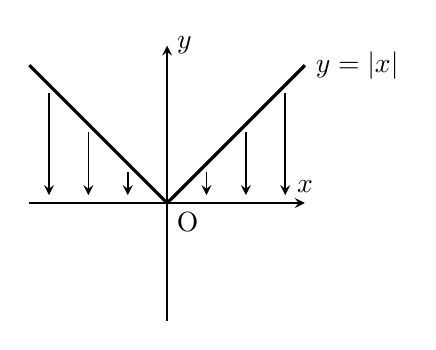
\begin{tikzpicture}
 \draw[->,>=stealth,semithick] (-1.75,0)--(1.75,0)node[above]{$x$}; %x軸
 \draw[->,>=stealth,semithick] (0,-1.5)--(0,2)node[right]{$y$}; %y軸
 \draw (0,0)node[below  right]{O}; %原点
 \draw[very  thick,domain=-1.75:1.75] plot(\x,{abs(\x)})node[right]{$y=|x|$};
 \draw[->,>=stealth,semithick] (0.5,0.4)--(0.5,0.1);
 \draw[->,>=stealth,semithick] (1.0,0.9)--(1.0,0.1);
 \draw[->,>=stealth,semithick] (1.5,1.4)--(1.5,0.1);
 \draw[->,>=stealth,semithick] (-0.5,0.4)--(-0.5,0.1);
 \draw[->,>=stealth,semithick] (-1.0,0.9)--(-1.0,0.1);
 \draw[->,>=stealth,semithick] (-1.5,1.4)--(-1.5,0.1);
\end{tikzpicture}
\end{wrapfigure}
$M$ は $\mathbb{R}^2$ の部分空間なのでHausdorff空間となる.

次に, 関数$y = |x|$ を$x$軸に射影する.

写像$\varphi$ を
\[\begin{array}{rccc}
\varphi \colon & M & \longrightarrow   & \mathbb{R} \\
        & \rotatebox{90}{$\in$} & & \rotatebox{90}{$\in$} \\
        & (x,|x|) & \longmapsto & x
\end{array}\]

とすると, 全単射は明らか. 射影なので連続. 逆写像$\varphi^{-1}$ の連続性も明らか. よって$\varphi$ は同相写像. 
以上より$M$は位相多様体.

\bigskip
\bigskip
\bigskip

(2)

\begin{wrapfigure}{r}{0pt} %図形を右側に
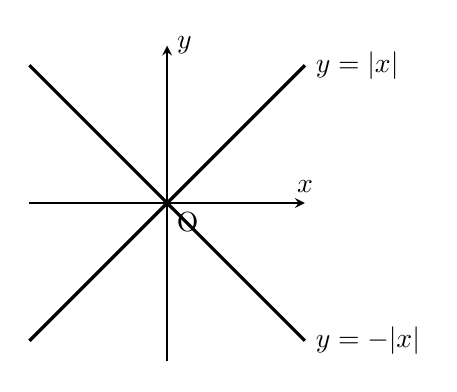
\begin{tikzpicture}
 \draw[->,>=stealth,semithick] (-1.75,0)--(1.75,0)node[above]{$x$}; %x軸
 \draw[->,>=stealth,semithick] (0,-2)--(0,2)node[right]{$y$}; %y軸
 \draw (0,0)node[below  right]{O}; %原点
 \draw[very thick,domain=-1.75:1.75] plot(\x,{abs(\x)})node[right]{$y=|x|$};
 \draw[very thick,domain=-1.75:1.75] plot(\x,{-abs(\x)})node[right] {$y=-|x|$};
\end{tikzpicture}
\end{wrapfigure}
$M$ は $\mathbb{R}^2$ の部分空間なのでHausdorff空間となるが, 原点$(0,0)$ 

では$\mathbb{R}^n$ の開集合と同相であるような開近傍が存在しない. 

実際, 原点の開近傍$U$ から$\mathbb{R}^n$ の開近傍$U'$ への同相写像

$$\varphi \colon U \longrightarrow U'$$

が存在すると仮定すると, これの制限写像

\hspace{5zw}
$\varphi|_{U-\{\bm{0}\}} \colon U - \{(0,0)\} \longrightarrow U'-\{\varphi(0,0)\}$

は同相写像となる. \ (全単射は明らか. 連続性は定義より)

\begin{wrapfigure}{r}{0pt}
      \begin{tikzpicture}
         \draw[name path = L1](0,0)--(2,2);
         \draw[name path = L2](2,0)--(0,2);
         \path[name  intersections={of=  L1  and  L2}]; 
         %L1とL2の交点の定義       
         \filldraw [fill=white] (intersection-1) circle 
         [radius= (0.1)];
         \draw(3,1)--(5,1);
         \filldraw [fill=white] (4,1) circle [radius=0.1];
         \draw(1,-0.5) node{$4$つ};
         \draw(4,-0.5) node{$2$つ};
         \draw(2.5,-1) node{連結成分の比較};
\end{tikzpicture}
\end{wrapfigure}
このとき, $U - \{(0,0)\}$ の連結成分は$4$ つであるが, $U'-\{\varphi(0,0)\}$ 

の連結成分を考えると, $n=1$ のときは$2$つ, $n \geqq 2$ のときは$1$つ

(i.e.連結) となるので同相写像が連結成分を保つことに矛盾する.

よって, $M$ は位相多様体とはならない.

$\left(  \begin{tabular}{l}
(1)との結果も踏まえると, この問題は位相多様体の和集合が\\
位相多様体にはならない例を表している.\\
ちなみに, 同じ次元の可微分多様体どうしの直和は\\
可微分多様体になることが知られている.
\end{tabular} \right)$

\bigskip

(3)

(2) と同様にして $M$ が位相多様体にならないことが示される.

\bigskip

\textbf{問7}

$\id_U$ は明らかに同相写像.

$f$ については, 定め方より全単射と連続性は明らかであり, $f^{-1}(x) = \sqrt[3]{x}$ となるような逆写像$f^{-1}$ は連続であるから$f$ は同相写像.

以上より, $(U, \id_U), \ (V, f)$ は$\mathbb{R}$ の座標近傍であり, $\mathbb{R} = U \cup V$ となるから $\{(U, \id_U), \ (V, f) \}$ は$\mathbb{R}$ の座標近傍系となる.

次に, $U \cap V = (-1, 1)$ において, $(V, f)$ から$(U, \id_U)$ への座標変換を考えると, 

\[\begin{array}{rccc}
\id_U \circ f^{-1} \colon & f (U \cap V) & \longrightarrow & \id_U (U \cap V) \\
& \rotatebox{90}{$\in$} & & \rotatebox{90}{$\in$} \\
& x & \longmapsto & \sqrt[3]{x} 
\end{array}
\]

となり, これは$x=0$ において微分可能でない.

$\because \ h \neq 0$ において, $\displaystyle \frac{\sqrt[3]{0+h} - \sqrt[3]{0}}{h}
= \frac{1}{h^{\frac{2}{3}}}$
となり, これは$h \to 0$ とすると収束しない.

よって, $\id_U \circ f^{-1}$ は$C^1$級ではない.

\bigskip

\textbf{問8}

$1$ 次元$C^{\infty}$ 級多様体$\mathbb{R}$ において, 
二つの座標近傍系

\begin{multicols}{2}
$\mathcal{S} = \{(\mathbb{R}, \ \id) \}$,

$\mathcal{T} = \{(\mathbb{R}, \ \varphi) \}$ \ \ 
を考えると, 

\vspace{0.4cm}

$\left( 
\begin{array}{rccc}
ただし, \ \varphi \ \colon & \mathbb{R} & \longrightarrow   & \mathbb{R} \\
        & \rotatebox{90}{$\in$} & & \rotatebox{90}{$\in$} \\
        & x & \longmapsto & x^3
\end{array}
\right)$
\end{multicols}

$\mathcal{S}, \ \mathcal{T}$ は$\mathbb{R}$ の$1$ 次元$C^{\infty}$ 級座標近傍系であるが, 
$\mathcal{S} \cup \mathcal{T}$ は$C^{\infty}$ 級座標近傍系ではない

(理由は問7と同様). \ よって, \ $\mathcal{S}$ と $\mathcal{T}$ は同値ではない.

\bigskip

\textbf{問9}

$\mathcal{S} \cup \mathcal{T}$ と $\mathcal{T} \cup \mathcal{U}$ が$C^{\infty}$ 級アトラスならば $\mathcal{S} \cup \mathcal{U}$ が $C^{\infty}$ 級アトラスになることを示す.

$\mathcal{M} := \mathcal{S} \cup \mathcal{T}$ とおくと, \ $\mathcal{M}$ の任意の元は $\mathcal{S}$ の元または$\mathcal{U}$ の元なので, \ $\mathbb{R}^m$ のある開集合と同相. よって, \ $M$ のアトラス$\{(\mathcal{M}_\alpha, \ \varphi_\alpha) \}_{\alpha \in \Lambda} \ (\Lambda は適当な添え字集合)$ を考えることができ, \ これの可微分性について考えていく.

略



\end{document}
